\documentclass{../../../fal_assignment}
\graphicspath{ {../../../} }

\usepackage{url}
\usepackage{graphicx}
\usepackage{amsmath}
\usepackage{varwidth}
\usepackage{xcolor}
\usepackage{algorithm}
\usepackage{algpseudocode}
\usepackage{listings}
\lstset{
	basicstyle=\footnotesize\ttfamily,
	tabsize=4,
	showstringspaces=false,
	breaklines=true,
	prebreak={\space\hbox{\textcolor{Gray}{$\hookleftarrow$}}},
	language=C++
}
\usepackage{enumitem}

\usepackage{tikz}
\usetikzlibrary{shapes.geometric, arrows}

\tikzstyle{flowchartnode} = [rectangle, minimum height=0.8cm, text centered, text width=3cm, draw=black, font=\small]
\tikzstyle{startstop} = [flowchartnode, rounded corners=0.4cm]
\tikzstyle{process} = [flowchartnode]
\tikzstyle{io} = [flowchartnode, trapezium, trapezium left angle=70, trapezium right angle=110, text width=2cm]
\tikzstyle{decision} = [flowchartnode, diamond, aspect=2, text width=2cm]
\tikzstyle{arrow} = [thick,->,>=stealth]

\title{COMP140 Worksheet A: Terminal Hacking}
\author{Brian McDonald \& Ed Powley}


\begin{document}

\maketitle

\section*{Introduction}

In this part, you will implement a version of the ``terminal hacking'' minigame from \emph{Fallout~4} (Bethesda, 2015); see Figure~\ref{fig:fallout_terminal}.
In this minigame you must guess a secret $n$-letter word, one of several options presented to you.
On choosing an option, you are told the \emph{likeness}: the number of letters which match the secret word (i.e.\ the same letter in the same position).
For example if the secret word is \texttt{HOUSE} and your guess is \texttt{MOUSE}, the likeness is $4$ out of $5$.
If your guess is \texttt{HOPES}, the likeness is $2$ out of $5$ (the letters \texttt{S} and \texttt{E} do not count as they are in the wrong positions).

The GitHub repository contains a project named \texttt{PartA\_TerminalHacking} for you to build upon.
This contains code to read words from a file, and choose the secret word and other words.
You will implement the rest of the game.


\begin{figure}[!h]
  	\centering
	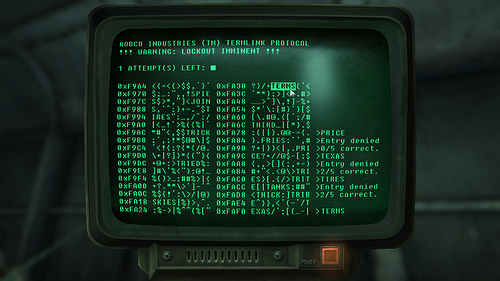
\includegraphics[width=0.8\textwidth]{fallout_terminal.jpg}
	\caption{A screenshot of the hacking minigame in \emph{Fallout~4}.
		Image from \protect\url{http://fallout.wikia.com/wiki/Terminal}.}
	\label{fig:fallout_terminal}
\end{figure}

\section{} \label{core-a-first}

Algorithm~\ref{alg:a_likeness} takes a guessed word and the secret word, and returns the likeness score as described above.

\textbf{Implement} the algorithm as a C++ function in \texttt{TerminalHacking.cpp}, choosing appropriate data types for the parameters, return value, and any variables.

\begin{algorithm}[t]
	\begin{algorithmic}
		\Procedure{GetLikeness}{guessedWord, secretWord}
		\State $\text{result} \gets 0$
		\For{$i = 0, 1, \dots, \text{secretWord.length} - 1$}
		\If{$\text{secretWord}[i] = \text{guessedWord}[i]$}
		\State increment result
		\EndIf
		\EndFor
		\State \textbf{return} result
		\EndProcedure
	\end{algorithmic}
	\caption{An algorithm for calculating the likeness score for the terminal hacking minigame.}
	\label{alg:a_likeness}
\end{algorithm}

\section{} \label{core-a-last}

\textbf{Implement} the main loop of the game, structured
according to the flowchart shown in Figure~\ref{fig:flowchart_a}.

\begin{figure}
	\begin{center}
		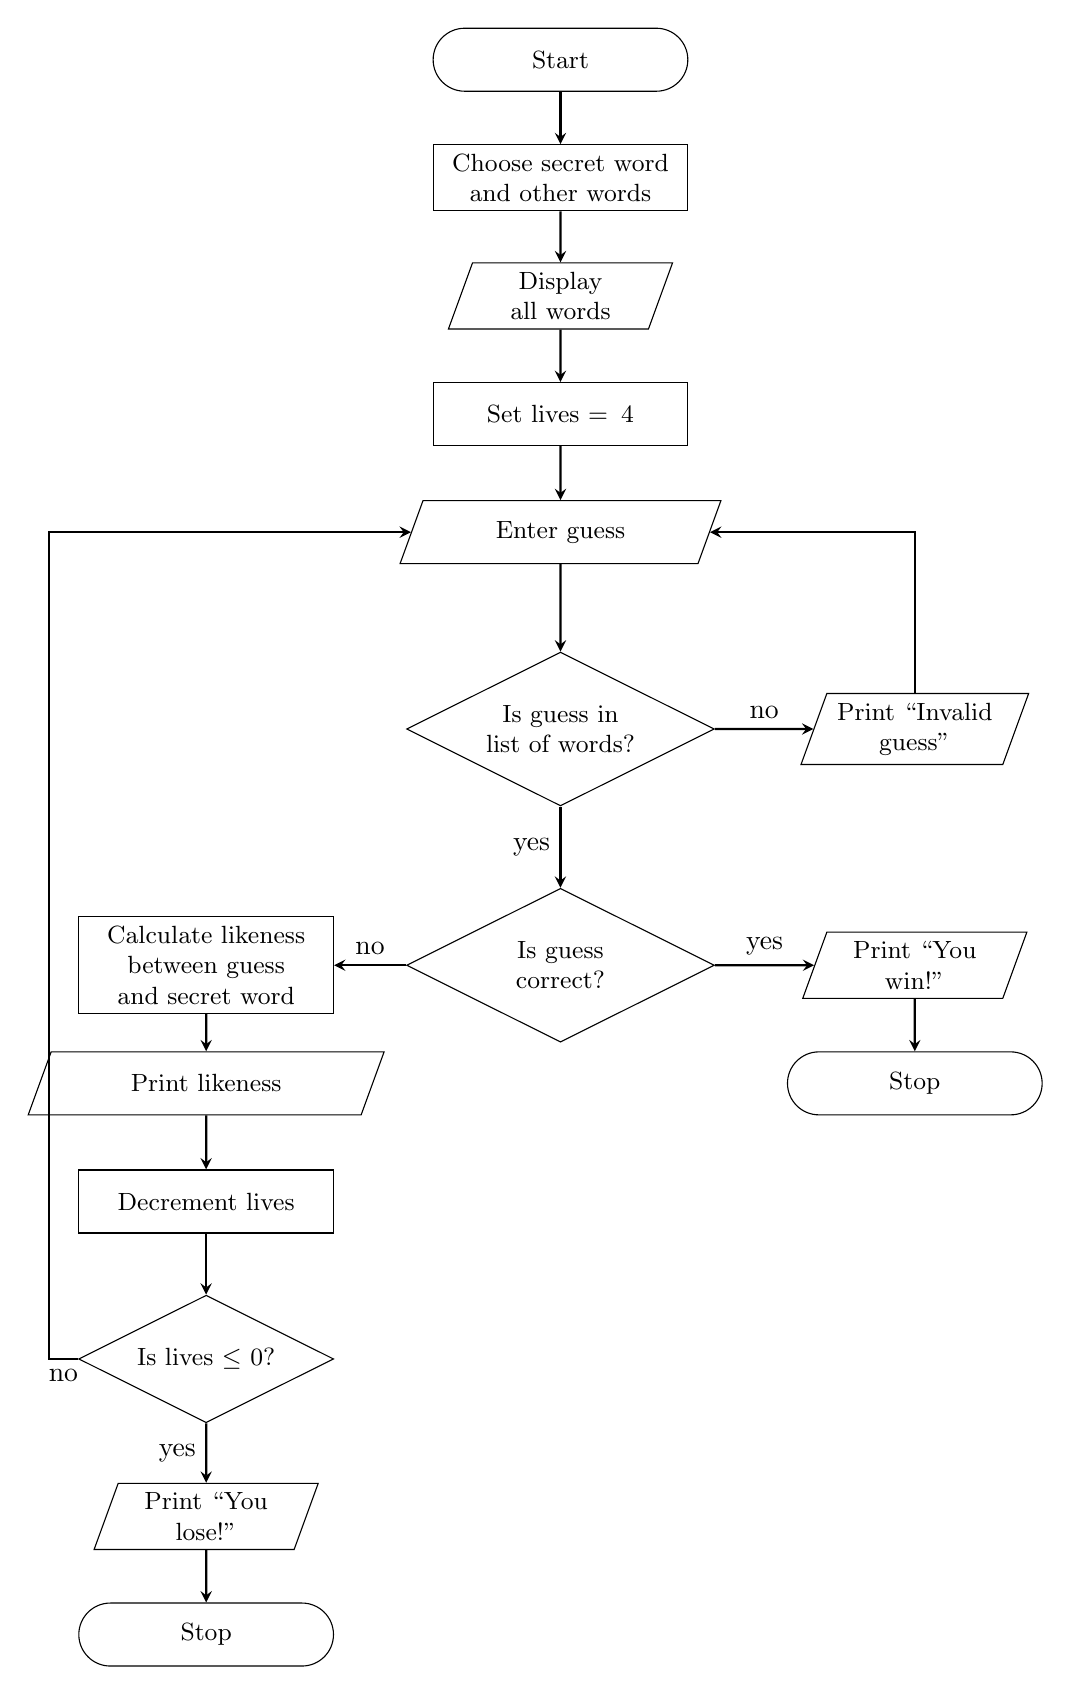
\begin{tikzpicture}[node distance=1.5cm]
		\node (start) [startstop] {Start};
		\node (choosewords) [process, below of=start] {Choose secret word and other words};
		\node (displaywords) [io, below of=choosewords] {Display all words};
		\node (initlives) [process, below of=displaywords] {Set lives $= 4$};
		\node (enterguess) [io, below of=initlives] {Enter guess};
		\node (isguessvalid) [decision, below of=enterguess, yshift=-1cm] {Is guess in list of words?};
		\node (guessinvalid) [io, right of=isguessvalid, xshift=3cm] {Print ``Invalid guess''};
		\node (isguesscorrect) [decision, below of=isguessvalid, yshift=-1.5cm] {Is guess correct?};
		\node (youwin) [io, right of=isguesscorrect, xshift=3cm] {Print ``You win!''};
		\node (stopwin) [startstop, below of=youwin] {Stop};
		\node (calclikeness) [process, left of=isguesscorrect, xshift=-3cm] {Calculate likeness between guess and secret word};
		\node (showlikeness) [io, below of=calclikeness] {Print likeness};
		\node (loselife) [process, below of=showlikeness] {Decrement lives};
		\node (isdead) [decision, below of=loselife, yshift=-0.5cm] {Is lives $\leq 0$?};
		\node (youlose) [io, below of=isdead, yshift=-0.5cm] {Print ``You lose!''};
		\node (stoplose) [startstop, below of=youlose] {Stop};
		\draw [arrow] (start) -- (choosewords);
		\draw [arrow] (choosewords) -- (displaywords);
		\draw [arrow] (displaywords) -- (initlives);
		\draw [arrow] (initlives) -- (enterguess);
		\draw [arrow] (enterguess) -- (isguessvalid);
		\draw [arrow] (isguessvalid) -- node[anchor=south] {no} (guessinvalid);
		\draw [arrow] (guessinvalid) |- (enterguess);
		\draw [arrow] (isguessvalid) -- node[anchor=east] {yes} (isguesscorrect);
		\draw [arrow] (isguesscorrect) -- node[anchor=south] {yes} (youwin);
		\draw [arrow] (youwin) -- (stopwin);
		\draw [arrow] (isguesscorrect) -- node[anchor=south] {no} (calclikeness);
		\draw [arrow] (calclikeness) -- (showlikeness);
		\draw [arrow] (showlikeness) -- (loselife);
		\draw [arrow] (loselife) -- (isdead);
		\draw [arrow] (isdead) -- node[anchor=east] {yes} (youlose);
		\draw [arrow] (youlose) -- (stoplose);
		\coordinate[left of=isdead, xshift=-0.5cm] (tmp1);
		\draw [arrow] (isdead) -- node[anchor=north] {no} (tmp1) |- (enterguess);
		\end{tikzpicture}
	\end{center}
	\caption{Flowchart for the Terminal Hacking game}
	\label{fig:flowchart_a}
\end{figure}

\section{Stretch goal} \label{stretch-a}

In the skeleton project, the words are chosen at random.
This may lead to instances of the game which are unsatisfying, for example where all words
have a low likeness score with respect to the secret word.

\textbf{Design} an improved word choosing algorithm.
Present your algorithm as pseudocode and/or a flowchart in your \texttt{readme.md} file on GitHub.

\textbf{Implement} your algorithm within your C++ project.

\section*{Submission instructions}

Begin by \textbf{forking} the GitHub repository at the following URL:

\url{https://github.com/Falmouth-Games-Academy/comp140-worksheetA}

You should complete a pull request before the hand-in on Friday by 5pm on Week 1. Feedback will be given in the pull request and in class.

\section*{Marking criteria}

Remember that \textbf{it is better to submit incomplete work than to submit nothing at all}. 

To demonstrate \textbf{basic competency}, complete the following:
\begin{itemize}
	\item \textbf{Timely Submission:} Obtain the marks for timely submission, you must submit (as a GitHub pull request).
	As with other worksheets, you may resubmit after these deadlines in order to collect extra correctness or quality marks.
	This is awarded as long as you submit \emph{something} for each part by the deadline,
	even if your submission has bugs or other issues.
\end{itemize} 

To demonstrate \textbf{basic proficiency}, complete the following:
\begin{itemize}
	\item \textbf{Achieve basic competency}
	\item \textbf{Complete} Algorithm \ref{core-a-first}. \textbf{Note:} You will not be penalised for trivial errors which do not
	affect the overall functioning of your programs
	\item Appropriate use of GitHub, with descriptive commit messages 
	\item Comments are used where appropriate, and are well written.
\end{itemize}

To demonstrate \textbf{novice competency}, complete the following:
\begin{itemize}
	\item Achieve \textbf{basic proficiency}
	\item \textbf{Complete} Algorithm \ref{core-a-last}. \textbf{Note:} You will not be penalised for trivial errors which do not
affect the overall functioning of your programs
	\item Your code is well formatted. Variable and function names are clear and descriptive.
\end{itemize}

To demonstrate \textbf{novice proficiency}, complete the following:
\begin{itemize}
	\item Achieve \textbf{novice competency}
	\item \textbf{Design} an improved word choosing algorithm 
\end{itemize}

To demonstrate \textbf{professional competency}, complete the following:
\begin{itemize}
	\item Achieve \textbf{novice proficiency}
	\item \textbf{Implement} an improved word choosing algorithm 
\end{itemize}


\end{document}
